\documentclass[titlepage]{article}

\usepackage{geometry}
\usepackage[utf8]{inputenc} % allow utf-8 input
\usepackage[T1]{fontenc}    % use 8-bit T1 fonts
\usepackage{hyperref}       % hyperlinks
\usepackage{url}            % simple URL typesetting
\usepackage{booktabs}       % professional-quality tables
\usepackage{amsfonts}       % blackboard math symbols
\usepackage{nicefrac}       % compact symbols for 1/2, etc.
\usepackage{microtype}      % microtypography
\usepackage{graphicx}
\usepackage{fancyhdr}
\usepackage{setspace}

\geometry{margin=1in}
\onehalfspacing

\title{\textit{Name for project} \\
    \large COMP4109 Group Project
}

\pagestyle{fancy}
\fancyhf{}
\lhead{COMP4109 Project Proposal}
\rfoot{\thepage}


% TODO: Fill in S#
\author{Adam Payzant \\
    \texttt{101082175} \\
    \and
    Kelvin Ratsamany \\
    \texttt{101120440}
    \and
    William So \\
    \texttt{101070267} \\
    \and
    Anders Sonstenes \\
    \texttt{101013731}
}

\begin{document}
    \maketitle

    % High level problem statement, goal, challenges, and what approaches have already been proposed
    \section{Introduction}

      For this project, we will be implementing a secure messaging and video app.
      The primary objective of this space is to provide a convenient way to send text messages and videos calls (both will be generalized as ``messages'') to others while not having to worry about the contents of the messages being breached.
      This has historically been a challenge as it's difficult, if not impossible, to guarantee transmission safety in your average modern network, as well as safely storing the messages after receiving them.
      Many attempts at solving this problem exist such as SMS, Apple's iMessage, WhatsApp, Signal, and many more.
      The majority of these solutions use some form encryption, passing through a central server, and then finally being sent along to their destination.
      In contrast, the Skype protocol system to not use a central server.
      However, we've noted all of these have notable failings or prioritized convenience over security.
      As a result, we've opted to use peer-to-peer transmission with end-to-end encryption to maximize security.

    % Give in-depth explanation of the problem. Talk about the failings of other secure messaging systems
    \section{Background}

      In the modern messaging space, all mainstream options have at least a few failings or trade-offs that fail the goal of absolute security.


      SMS (conventional texting) is highly susceptible to transmission interception, does not transmit securely, and is easily traced back to the sender/recipient.
      \footnote{\url{https://www.popularmechanics.com/technology/security/a29789903/what-is-sms/}}
      Apple's iMessage offers end-to-end encryption (which means the message is sent encrypted and can only be unencrypted by the recipient), but the messages are still stored on Apple's servers and are only usable on Apple devices.
      In 2021, WhatsApp changed their privacy policy to allow more sharing of user data towards Facebook, which can include some messages.
      \footnote{\url{https://www.androidpolice.com/2021/01/12/whatsapps-new-terms-of-service-are-a-facebook-or-die-ultimatum/}}
      Skype, while offering peer-to-peer messaging, utilized the vulnerable RC4 encryption protocol creating a whole new slew of security risks.
      Even the poster child of secure messaging apps, Signal, has trade-offs as data still goes through their servers, can be stored on their servers, and prevents anonymity by requiring a phone number.
      \footnote{\url{https://nakedsecurity.sophos.com/2020/05/22/signal-secure-messaging-can-now-identify-you-without-a-phone-number/}}\\

      Based on these failings, our app aims to mitigate them by following these principles:
      \begin{enumerate}
          \item Message Security - A message should be encrypted before sending and can only be decrypted by the recipient upon receiving the message
          \item Safe Storage - Messages should be stored in safe way and should strive to guarantee complete deletion upon request
          \item Anonymity - Users should be anonymous in the eyes of the system. This increases user safety by increasing the work factor to attack an individual
      \end{enumerate}

      Each of these principles are vital for a number of reasons.
      Message security is vital as there is no practical way to guarantee secure transmission over the internet.
      When sending unsecure data, a Man-in-the-Middle Attack, an attack where data in transit is intercepted, read, then send to the intended target, can easily collect user information.
      \footnote{\url{https://www.csoonline.com/article/3340117/what-is-a-man-in-the-middle-attack-how-mitm-attacks-work-and-how-to-prevent-them.html}}
      Message security can be achieved by using a public-key encryption method, where the data is encrypted using the recipient's public key, and only decrypted by the recipient's secret private key.
      This will mitigate any attacks occurring during data transmission.
      Safe Storage is critical as attacks can still occur after the message has been received.
      Storing messages unencrypted posing the risk of that storage service being broken into, and allows an attack to collect the contents.
      In addition, even if the stored data is encrypted, it may not provide sufficient work factor, meaning an attack must take more effort than the data is worth, to actually be considered secure.
      \footnote{van Oorschot, Paul C. \textit{Computer Security and the Internet: Tools and Jewels}. Springer, 25 Sept 2019}
      Not to mention, while an encryption method today may be considered secure, in 5 years the method may no longer be considered to be a sufficient work factor.
      Finally, anonymity is vital to making a secure messaging system.
      Making users anonymous in the eyes of the system adds yet another layer of security should the system be breached.
      Doing so increases the work required for an attacker to pinpoint a user's identity, making a security breach less damaging.

    % Talk about the architecture of our system
    \section{System Description}

      \subsection{High Level Architecture}

      \begin{center}
          \begin{figure}[!ht]
              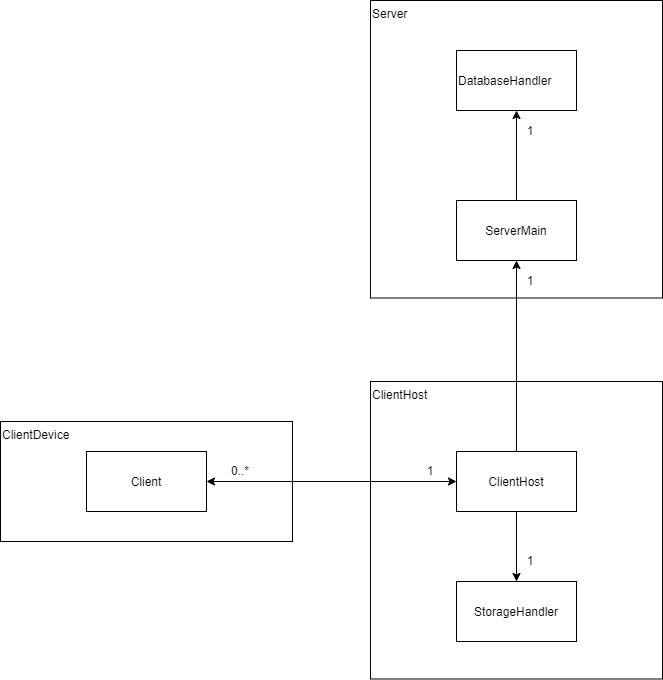
\includegraphics[scale=.5]{graphics/arch.png}
              \label{componenets}
              \caption{A diagram of the components in the system}
          \end{figure}
      \end{center}

      This system will utilize a peer-to-peer system, with a central server to connect users.
      When a user wants to send a message, it first sends a request to the server for the user's public key and IP (individual clients do not store this to simplify key changing process).
      After recieving this information, the user can then use the key to encrypt the data, either a message or video call, and send it directly to the recipient.
      A sequence diagram of what a sending a message would be like can be seen in figure \ref{sequence}.
      From our current research, video calling should effectively be the same, but concurrently be recieving a message as well.
      All messages will be securely stored by both the sender and recipient.

      \begin{center}
          \begin{figure}[!ht]
              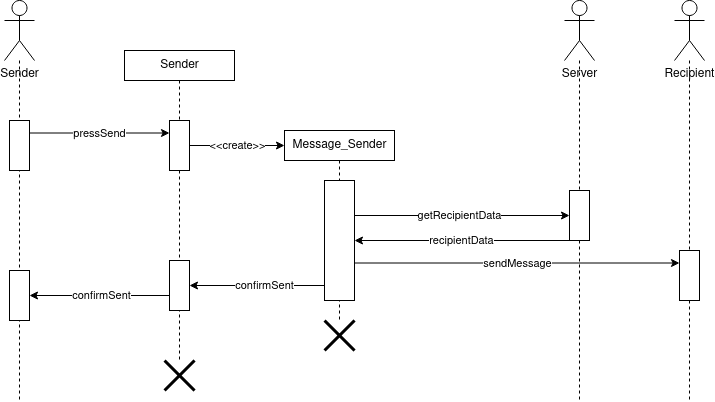
\includegraphics[scale=.5]{graphics/SequenceDiagram.png}
              \label{sequence}
              \caption{Messaging sequence diagram}
          \end{figure}
      \end{center}

      The client's architecture is one of the more interesting sides of this project.
      Most of the best messaging apps offer some cross-platform support, and conversation histories will be shared between devices.
      We wanted to bring this feature into our own app, but the P2P nature of messaging made this challenging.
      To get around this, we've opted to have each client have their own host system.
      While this decision makes it no longer a true peer-to-peer system, it's a trade-off we've deemed acceptable and it can still remain decentralized from our own servers.
      This allows the modern convenience of linked devices while also keeping data off unknown servers.
      With the addition of the host, the flow of a message can be seen in figure \ref{clientHost}.
      As shown, a message sent from a client's device is first sent to their host.
      As previously shown, the host will access the central server to get the recipient's IP, then send the message along to the recipient's host.
      The sender's host will also update all device's conversation to reflect the new message.
      When the host receives the message, it will then distribute it to all client devices.
      However, as seen in the diagram, this hierarchy does not occur for video calling.
      The host structure could a decent amount of latency.
      While this isn't a critical for message sending, it would make video calling sub-optimal, especially if any link in the chain has poor network speeds.
      To avoid this issue, a direct link is established between the two devices video calling.

      \begin{center}
          \begin{figure}[!ht]
              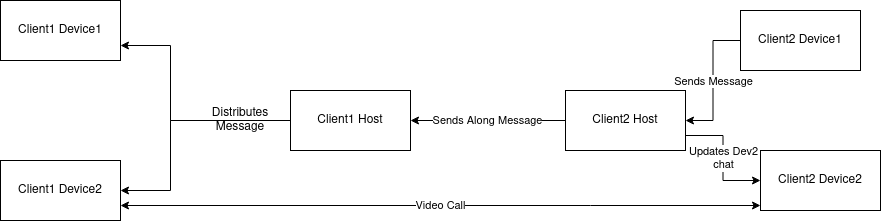
\includegraphics[scale=.5]{graphics/clientHost.png}
              \label{clientHost}
              \caption{The flow of one of Client 2's devices sending a message and how a video call is performed}
          \end{figure}
      \end{center}

      Compared to the client architecture, the central server's architecture is fairly boring.
      This server's primary goal is to manage users.
      To this end, it handles user registration, tracks user's public key and IP, and serves it to user request.
      When a user registers for the system, they will create a username and key pair and provide a host IP.
      The key will be generated client side (will be obscured from the user for quality of life) so that the server can never know the secret private key.
      User authentication can be handled by just sending an authentication token encrypted with the users public key, and expecting the unencrypted token to be sent with subsequent requests.
      The actions of the server are strictly triggered by user requests and all will access the database.
      The use cases of the server can be seen in figure \ref{serverUse}.

      \begin{center}
          \begin{figure}[!ht]
              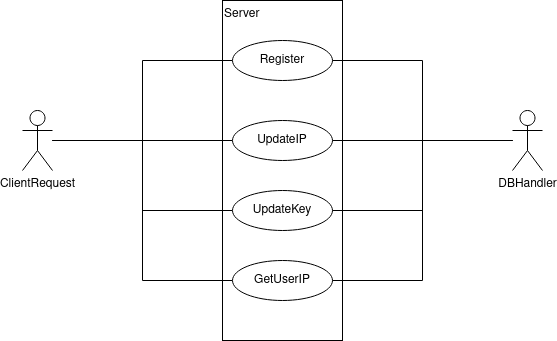
\includegraphics[scale=.5]{graphics/ServerUseCase.png}
              \label{serverUse}
              \caption{A use case diagram of user requests to the server}
          \end{figure}
      \end{center}

    \subsection{Tech Stack}

      The current tech stack planned for this project is to use gRPC for the transmission of data.
      For server side storage we will likely use a noSQL database like MongoDB as it will be more performantly scalable because our data will not be relational.
      We have no final decision on the language to implement in.
      We are currently leaning towards Go for the server and client hosts, application implementations may vary however.
      Depending on what we choose to support, some languages may be optimal for different OS's, this is why gRPC was an intentional choice to maintain compatibility between languages.

      \subsection{Stretch Targets}

      This project seems relatively easy, but without more in-depth research, the apparent ease may be deceptive.
      To add some depth to this project if it turns out to be too simple, while also giving some leeway in case it turns out to be harder than expected, we've added some stretch goals.
      \begin{itemize}
          \item Provide client hosting, just make individual docker containers server-side
          \item For the host, make an additional program with root permissions to read the private key, increasing security of the key
          \item Support more than just Linux
          \item Do some kind of checksum for the messages to guarantee conversation's integrity (not sure how feasible that is)
          \item Include ability to allow/block particular public keys of other users
      \end{itemize}

      \subsection{Potential Challenges}

      Video chatting will likely be the most difficult part of this project.
      While messaging seems like a relatively simple process using gRPC and some off-the-shelf encryption libraries, video streaming seems like more of a challenge.
      Due to some limitations of gRPC, we may need to use a different technology for this, but that will require research beyond this proposal.
      The actual encryption method for video is relatively trivial with some more time tested libraries for encryption and processing.

      \subsection{Architectural Failings}

      Unfortunately, this system architecture cannot fully maintain user anonymity.
      While this system does store a user's IP and a username, the username can be fully anonymous and the IP can still be setup through a proxy so identifying information can be reduced.
      Because both parties in a conversation should have the records, there's no guarantee if one deletes the message the other also is.
      We believe there has still been adequate risk mitigation, as only those two should be able to access the messages.

    % Do some timeline for our development
    \section{Implementation Plan}
    
    The following is an outline for the implementation of features for the application over time. \\

	\begin{tabular}{l r l}
		\textbf{Task Name}	& \textbf{Time allotted} & \textbf{Description}\\
		gRPC Protocol		& Week 0 - 1 & Develop the implementation of gRPC used for application\\
		Server DB  			& Week 0 - 1 & Build the Database that stores Data on Connection Server\\
		Server Backend 		& Week 0 - 1 & Create a server used to advertise active Clients\\
		Client Backend 		& Week 1 - 2 & Create the backend for the client application\\
		Client Messaging 	& Week 2 - 3 & Finalize the ability to send text messages using the application\\
		Client Video 		& Week 3 - 5 & Implement the ability for video calling between users\\
		Stretch Goals 		& Week 5 - 8 & Work on implementing stretch goals (work on unfinished tasks if applicable)\\
		Front End  			& Week 0 - 8 & Develop the front-end of the application\\
		Video Demo	 		& Week 5 - 8 & Produce Video for demonstration \\	
	\end{tabular}

	\begin{center}
		\begin{figure}[!ht]
			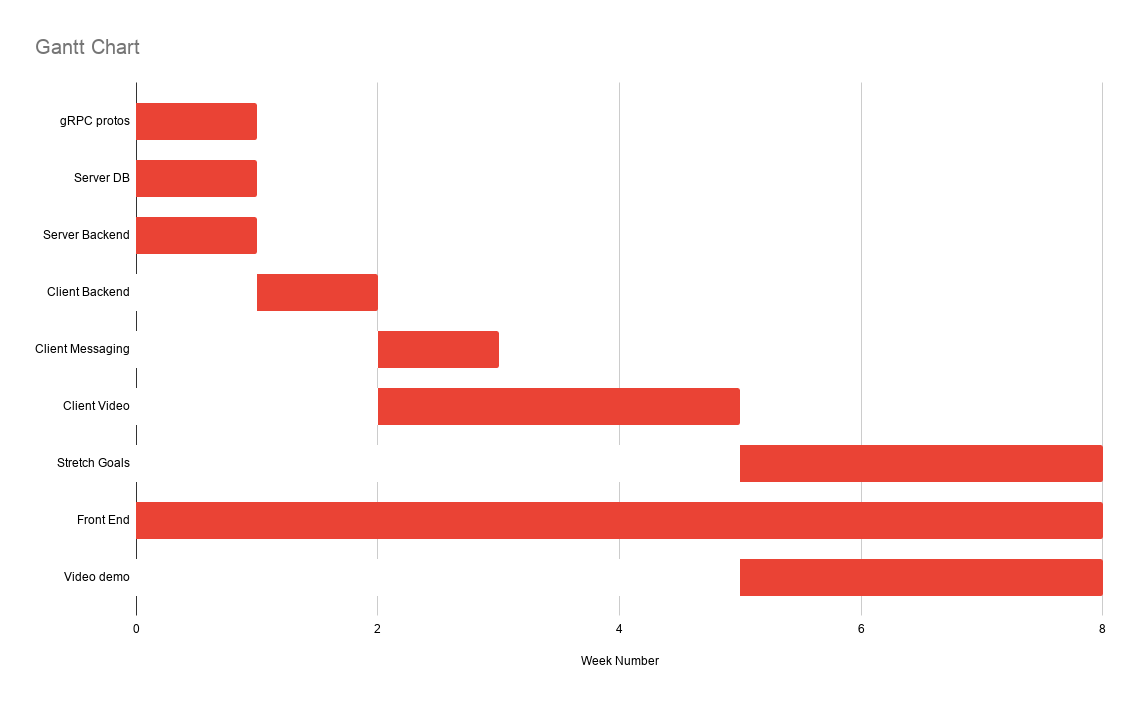
\includegraphics[scale=.35]{graphics/GanttChart.png}
			\caption{A gantt table for our development timeline}
		\end{figure}
	\end{center}
	



\end{document}
